\documentclass[letterpaper,11pt]{article}

\usepackage{latexsym}
\usepackage[empty]{fullpage}
\usepackage{titlesec}
\usepackage{marvosym}
\usepackage[usenames,dvipsnames]{color}
\usepackage{verbatim}
\usepackage{enumitem}
\usepackage[hidelinks]{hyperref}
\usepackage{fancyhdr}
\usepackage[english]{babel}
\usepackage{tabularx}
\usepackage{fontawesome5}
\usepackage{multicol}
\setlength{\multicolsep}{-3.0pt}
\setlength{\columnsep}{-1pt}
\input{glyphtounicode}

%new packages

\usepackage{fontenc}
\usepackage{amsmath}
\usepackage{amssymb}
\usepackage{graphicx}



%----------FONT OPTIONS----------

\pagestyle{fancy}
\fancyhf{} % clear all header and footer fields
\fancyfoot{}
\renewcommand{\headrulewidth}{0pt}
\renewcommand{\footrulewidth}{0pt}

% Adjust margins
\addtolength{\oddsidemargin}{-0.6in}
\addtolength{\evensidemargin}{-0.5in}
\addtolength{\textwidth}{1.19in}
\addtolength{\topmargin}{-.7in}
\addtolength{\textheight}{1.4in}

\urlstyle{same}

\raggedbottom
\raggedright
\setlength{\tabcolsep}{0in}

% Sections formatting
\titleformat{\section}{
  \vspace{-4pt}\scshape\raggedright\large\bfseries
}{}{0em}{}[\color{black}\titlerule \vspace{-5pt}]



% Ensure that generate pdf is machine readable/ATS parsable
\pdfgentounicode=1

%-------------------------
% Custom commands
\newcommand{\resumeItem}[1]{
  \item\small{
    {#1 \vspace{-2pt}}
  }
}

\newcommand{\classesList}[4]{
    \item\small{
        {#1 #2 #3 #4 \vspace{-2pt}}
  }
}

\newcommand{\resumeSubheading}[4]{
  \vspace{-2pt}\item
    \begin{tabular*}{1.0\textwidth}[t]{l@{\extracolsep{\fill}}r}
      \textbf{#1} & \textbf{\small #2} \\
      \textit{\small#3} & \textit{\small #4} \\
    \end{tabular*}\vspace{-7pt}
}

\newcommand{\resumeSubSubheading}[2]{
    \item
    \begin{tabular*}{0.97\textwidth}{l@{\extracolsep{\fill}}r}
      \textit{\small#1} & \textit{\small #2} \\
    \end{tabular*}\vspace{-7pt}
}

\newcommand{\resumeProjectHeading}[2]{
    \item
    \begin{tabular*}{1.001\textwidth}{l@{\extracolsep{\fill}}r}
      \small#1 & \textbf{\small #2}\\
    \end{tabular*}\vspace{-7pt}
}


\newcommand{\resumeSubItem}[1]{\resumeItem{#1}\vspace{-4pt}}

\renewcommand\labelitemi{$\vcenter{\hbox{\tiny$\bullet$}}$}
\renewcommand\labelitemii{$\vcenter{\hbox{\tiny$\bullet$}}$}

\newcommand{\resumeSubHeadingListStart}{\begin{itemize}[leftmargin=0.0in, label={}]}
\newcommand{\resumeSubHeadingListEnd}{\end{itemize}}
\newcommand{\resumeItemListStart}{\begin{itemize}}
\newcommand{\resumeItemListEnd}{\end{itemize}\vspace{-5pt}}



\begin{document}
\fontfamily{cmr}\selectfont
\begin{center}
\parbox{3.0cm}{%
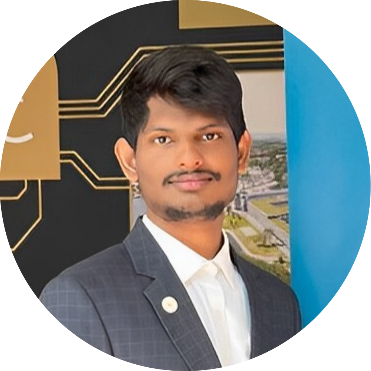
\includegraphics[width=2.7cm,clip]{images/resume_pic_m.png}}
}
\parbox{\dimexpr\linewidth-3.8cm\relax}{
\vspace{-20pt}
\begin{tabularx}{\linewidth}{L r} \\
    {\Huge \scshape  Venkata Sai Yakkshit Reddy Asodi}~
    \href{https://www.cedzlabs.com/yakkshit}{\vspace{1pt}}\\
      Berlin, Germany \\ \vspace{1pt}
     \small \raisebox{-0.1\height}\faPhone\ +91 9493006444 ~ \href{mailto:saiyakkshit2001@gmail.com}{\raisebox{-0.2\height}\faEnvelope\  {saiyakkshit2001@gmail.com}} ~ 
    \href{https://linkedin.com/in/yakkshit/}{\raisebox{-0.2\height}\faLinkedin\ {yakkshit}}  ~
    \href{https://yakkshit.com/}{\raisebox{-0.2\height}\faGlobe\ {yakkshit.com}}  ~
    \href{https://github.com/yakkshit}{\raisebox{-0.2\height}\faGithub{ yakkshit}}
    \vspace{-8pt}
\end{tabularx}
}
\end{center}

\vspace{-23pt}
\href{https://www.yakkshit.com/#details}{\section{Summary \faLink}
Innovative Full Stack Engineer with expertise in TypeScript and Next.js, specializing in building user-centric web applications. Proven track record of leading technical initiatives and developing scalable solutions. Passionate about creating intuitive digital experiences and driving product innovation through technology. Strong background in both frontend and backend development with experience in startup environments.}

\section{\href{https://www.linkedin.com/in/yakkshit/details/skills/}{Technical Skills} \faLink}
\begin{itemize}[leftmargin=0.15in, label={}]
\small{\item{
\textbf{Frontend - }{Next.js, TypeScript, React.js, HTML5, CSS3, TailwindCSS} \\
\textbf{Backend - }{Node.js, Express, PostgreSQL, MongoDB, RESTful APIs} \\
\textbf{Tools - }{Git, Docker, AWS, Vercel, Agile/Scrum} \\
\textbf{Testing - }{Jest, React Testing Library, Cypress}\\
}}
\end{itemize}
\vspace{-10pt}

\section{Experience \faLinkedin}
\resumeSubHeadingListStart

\resumeSubheading
{\large Circleup AG \faBuilding}{December 2023 -- July 2024}
{Lead Full Stack Engineer}{\faMapMarker \hspace{0.1cm} Zurich, Switzerland}\\
\vspace{10pt}
\textbf{Responsibilities:}
\resumeItemListStart
\vspace{-10pt}
\resumeItem{Led the development of a TypeScript-based web application using Next.js, implementing features that improved user engagement by 45\%}
\resumeItem{Designed and implemented scalable database architecture using PostgreSQL, handling data for 50,000+ active users}
\resumeItem{Mentored junior developers and established best practices for code quality and testing, reducing bug reports by 60\%}
\resumeItemListEnd
\vspace{-3pt}
\textbf{Environment:}\emph{Next.js, TypeScript, PostgreSQL, AWS, Docker}

\resumeSubheading
{Cedzlabs \faBuilding}{March 2023 -- July 2024}
{Full Stack Developer}{\faMapMarker \hspace{0.1cm} Berlin, Germany}\\
\vspace{10pt}
\textbf{Responsibilities:}
\vspace{-10pt}
\resumeItemListStart
\resumeItem{Developed and maintained user-friendly interfaces using React and TypeScript, achieving a 98\% user satisfaction rate}
\resumeItem{Implemented automated testing strategies resulting in 85\% test coverage and 40\% fewer production bugs}
\resumeItemListEnd
\vspace{-3pt}
\textbf{Environment:}\emph{React, TypeScript, Node.js, MongoDB, Jest}

\resumeItem{\textbf{\href{https://linkedin.com/in/yakkshit}{Checkout my other experiences by clicking here}}}
\vspace{-5pt}

\section{Projects \faGithub}
\vspace{-5pt}
\resumeSubHeadingListStart
\resumeProjectHeading
{\textbf{\href{https://ui.cedzlabs.com/resume}{PawCare Platform}} $|$ \emph{Next.js, TypeScript, PostgreSQL}}{2024}\\
\vspace{6pt}
\textbf{Description:}
\vspace{-5pt}
\resumeItemListStart
\resumeItem{Developed a comprehensive pet care management system using Next.js and TypeScript. Implemented features including appointment scheduling, medical record management, and real-time notifications. Integrated with PostgreSQL for robust data management and implemented responsive design for optimal user experience across devices.}
\resumeItemListEnd
\vspace{4pt}
\textbf{Tools:}\emph{
Next.js, TypeScript, PostgreSQL, TailwindCSS, Vercel}
\vspace{-10pt}

\resumeProjectHeading
{\href{https://yakkshit.com}{\textbf{Health Monitor Dashboard}} $|$ \emph{React, Node.js, MongoDB}}{2023}\\
\vspace{6pt}
\textbf{Description:}
\vspace{-5pt}
\resumeItemListStart
\resumeItem{Built a real-time health monitoring dashboard using React and Node.js. Implemented features for data visualization, alert systems, and automated reporting. Utilized MongoDB for flexible data storage and real-time updates.}
\resumeItemListEnd
\vspace{4pt}
\textbf{Tools:}\emph{React, Node.js, MongoDB, Socket.io, Chart.js}
\vspace{-12pt}

\section{Achievements / Contributions}
\resumeSubHeadingListStart
\resumeItemListStart
\resumeItem{Led migration of legacy system to Next.js, improving performance scores by 65\%}
\resumeItem{Contributed to open-source TypeScript libraries with 500+ GitHub stars}
\resumeItem{Reduced application loading time by 70\% through implementation of dynamic imports and code splitting}
\resumeItemListEnd

\resumeSubHeadingListEnd
\textbf{Strengths:}\emph{Technical Leadership, Problem-solving, User-Centric Development, Agile Methodologies} \\
\textbf{Education:}\emph{Bachelor of Technology in Computer Science, JNTU Hyderabad (2019-2023)} \\
\textbf{Languages:}\emph{Telugu - Native $|$ English - Fluent $|$ Hindi - Fluent $|$ German - Intermediate}

\vspace{10pt}
\end{document}